% thios section describes the computational image complexity analysis

The theory framework section meticulously examined the architectural evolution, revealing a recurring cycle oscillating between complex and simple styles.
Given the recent technological advancements and contemporary architectural trends, there is a compelling indication that the present era is poised for a shift toward complexity, countering the preceding Modernist movement characterized by minimalism and simplicity.

In pursuit of validating this hypothesis, we developed a Computational Image Complexity Analysis (CICA) system.
Our primary objective was to not only empirically validate the trends in architectural complexity suggested by our theoretical analysis but also to create a quantifiable metric.
This metric would play a crucial role in evaluating and ranking the 3D-modeled facades intended for use in the Virtual Reality experience.

The Computational Image Complexity  Analysis (CICA) system is a Python function that assesses complexity by quantifying the number of elements within a building's design.
The higher the count of elements, the higher the assigned complexity score, and vice versa.
This approach draws inspiration from Venturi et al.'s reflection on complexity, as articulated in their work\cite{Venturi1977}.
They posited that a building's complexity could be gauged by the time it takes to mentally process and form a coherent image of its constituent elements.
This fundamental concept underpins the CICA system's methodology(Figure\ref{fig:ImageComplexityAnalysisFlowchart}).

%% Figure Computational Image Compexity Analysis (CICA) System flowchart
    \begin{figure}[!htb]
      \centering
      % trim=left 190 down 250 right 150 top5
      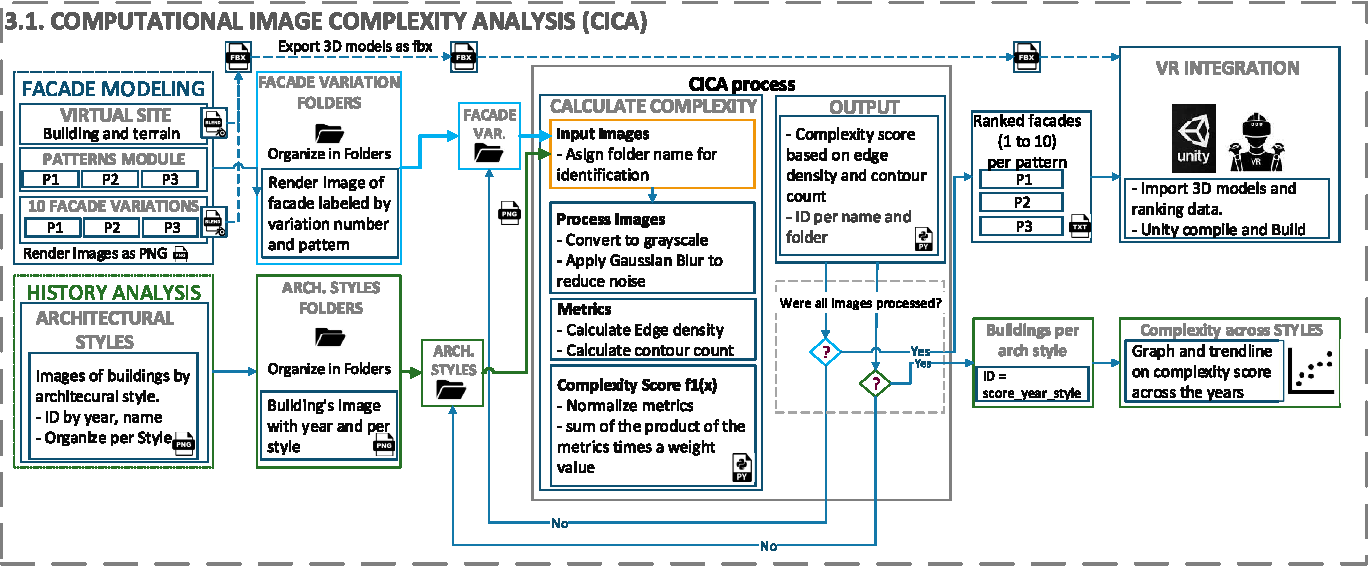
\includegraphics[width= \linewidth, trim=0 0 0 0, clip]{Images/ImageComplexityAnalysisFlowchart}
      \caption{Flowchart illustrating the applications of Computational Image Complexity Analysis, including its role in analyzing complexity scores for historical architectural styles and ranking modeled facades for the VR Building Complexity System.}
      \label{fig:ImageComplexityAnalysisFlowchart}
    \end{figure}

The Computational Image Complexity Analysis (CICA) system as shown in Figure\ref{fig:ImageComplexityAnalysisFlowchart} works by using building images as input, subsequently processing these images to enhance contrast and minimize noise, thereby improving the recognition of individual elements within the building's design.

The system employs a method of complexity quantification based on edge density.
A pronounced edge within the image can be associated with a distinct element of the building, and in the case of more intricate structures, this script interprets such edges as separations denoting additional elements.

Edge detection is a critical step in our Computational Image Complexity Analysis (CICA) system, performed using the Canny Edge Detection algorithm\cite{OpenCV2023}.
This algorithm, readily accessible in Python through OpenCV (cv2.Canny function), is designed for computer vision tasks and excels at identifying edges within an image.
It achieves this by identifying regions of the image where there is a rapid change in intensity, often corresponding to object boundaries or significant features.
The outcome of this process is an abstraction that highlights the most relevant features of the building, as demonstrated in Figure\ref{fig:CannyEdgePlotHistory}.

%%Figure Canny Edge of historic buildings
     \begin{figure}[htb]
          \centering
          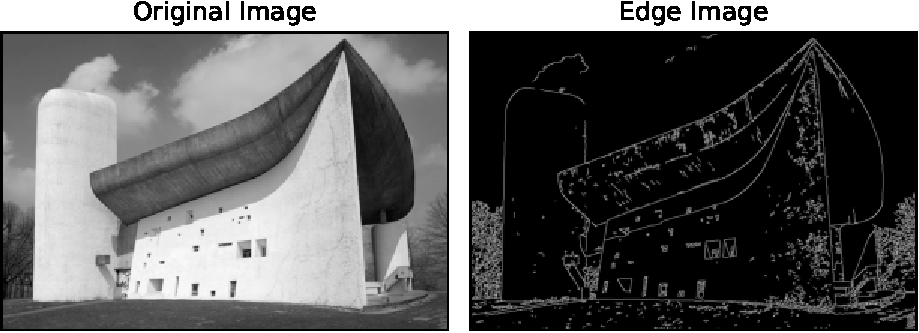
\includegraphics[width= \linewidth]{Images/CannyEdgePlotHistory}
          \caption{Comparison of the original image of Chapelle Notre-Dame-du-Haut de Ronchamp, constructed in 1955 (left), with its corresponding Edge Detection Plot image (right) generated using the cv2.Canny function from OpenCV in Python. The Edge Detection Plot illustrates key architectural features and edge density within the building's design.}
          \label{fig:CannyEdgePlotHistory}
        \end{figure}

The edge density is subsequently computed by dividing the number of non-zero (edge) pixels in the edges image by the total number of pixels in the original image.
This calculation provides a measure of how much of the image consists of edges, resulting in an edge density score that serves as a proxy for complexity.

In essence, the CICA system quantifies the complexity of a building based on the presence and density of edges in its image.
A higher edge density typically indicates greater complexity or intricacy in the building's design, making it a valuable metric for our analysis.

Having outlined the development and purpose of the Computational Image Complexity Analysis (CICA) system, we will now delve into its application.

%! section on CICA applied to historical analysis
First, we will employ the CICA system to quantify the complexity score for a selection of renowned buildings representing different architectural eras and styles (Figure \ref{fig:CannyEdgePlotHistory}).

This comprehensive dataset includes a total of 180 buildings, meticulously organized according to architectural style, with an average of 10 buildings per style, each labeled with its name and year of construction (as illustrated in Figure \ref{fig:ImageComplexityAnalysisFlowchart}).

This analytical endeavor will culminate in the creation of a scatter graph, thoughtfully color-coded to distinguish architectural styles, and accompanied by a trendline.
Together, these visualizations aim to provide a clear depiction of the trends in complexity across the years.

By categorizing data per architectural style and era, we intend to substantiate whether a cyclical pattern indeed exists in architectural design throughout history.
Furthermore, this analysis will offer empirical evidence regarding the contemporary architectural shift towards more intricate and complex designs, aligning with the conclusions drawn from our theoretical examination.

%!Section on CICA applied for 3d modeled facades ranking

With the first application of the Computational Image Complexity Analysis (CICA) system shedding light on the historical trends in architectural complexity, we now pivot our focus to the second application of this tool.
In this phase, the CICA system will be harnessed for a distinct purpose: the ranking of 3D-modeled facades (Figure\ref{fig:CannyEdgePlotRender}).

As part of our upcoming Virtual Reality (VR) experiment, participants will interact with facades showcasing varying levels of complexity.
To facilitate this experiment, the CICA system will evaluate the complexity of 10 facade variations for each of the three distinct patterns modeled in Blender.
These variations will be ranked into 10 levels of complexity.
During the VR experience, participants will select the complexity level they find most comfortable, thereby allowing us to discern user preferences and tolerance thresholds with precision.

%%Figure Canny Edge of render buildings
     \begin{figure}[htb]
          \centering
          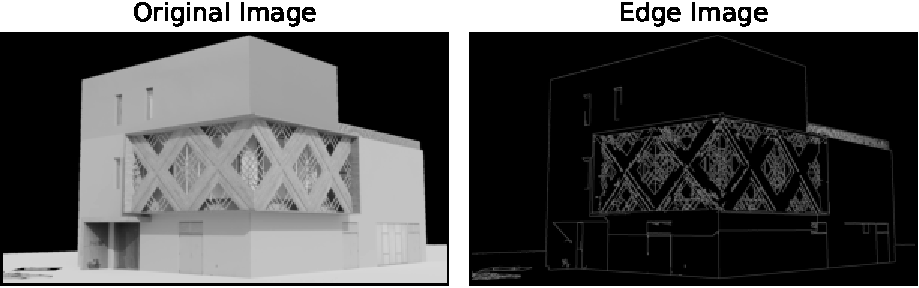
\includegraphics[width= \linewidth]{Images/CannyEdgePlotRender}
          \caption{Comparison of the original image of render of facades variation modeled in blender for the VR complexity analysis system used on this research(left), with its corresponding Edge Detection Plot image (right) generated using the cv2.Canny function from OpenCV in Python. The Edge Detection Plot illustrates key architectural features and edge density within the 3D modeled facade's design.}
          \label{fig:CannyEdgePlotRender}
        \end{figure}

%%%%%%%%%%%%%%%%%%%%%%%%%%%%%%
%%there migh be need for a transition paragraph into VR